% ============================================================================
% Drop-in LaTeX for Section 7.1 (revised) + a new betting-strategy subsection.
%
% Preamble requirements (add to the manuscript preamble if not already present):
%   \usepackage{booktabs}
%   \usepackage{multirow}   (used by the betting-strategy table only)
%
% Table/figure paths below are relative to the repo root
% (multi-change-points/). Adjust the prefix (or set \graphicspath) to match
% wherever the manuscript source actually lives.
%
% NOTE ON CONTENT: this revision corrects three discrepancies between the
% previous Section 7.1 prose and simulations/joint_simulations.R, all
% resolved in favor of matching the text to the already-generated results
% (no re-simulation was needed):
%   1. The "misspecified" detector plugs in mu1 + 0.1 (a fixed additive
%      offset applied to every coordinate of mu1, including unaffected
%      streams under sparse change) -- NOT mu1/2 or a pre/post interpolation.
%   2. CAD/ARL are averaged over 300 replications, not 500.
%   3. EWMA-AGRAPA uses c = 0.75 (the package default; c is not overridden
%      in joint_simulations.R), not c = 0.9.
% It also now documents the independent/correlated grid dimension that was
% already in joint_simulations.R (and feeds joint_effect_of_dependence.png)
% but was previously unmentioned in the prose.
% ============================================================================


% ----------------------------------------------------------------------------
% REVISED Section 7.1 (replace the existing paragraph with this block)
% ----------------------------------------------------------------------------

\subsection{Joint detection}

We evaluate the efficiency of our proposed detectors in a simulation study of VAR($p$) processes:
\[
\bm{X}_t = \bm{\mu} + \sum_{j=1}^p \bm{\phi}_j^T (\bm{X}_{t-j} - \bm{\mu}) + \bm{\varepsilon}_t.
\]
The fact that $\bm{\phi}_j^T$ are written as vectors indicates there is no cross-stream Granger
causality. We gather the coefficients into a $K \times p$ matrix
$\bm{\Phi} = \bm{\Phi}_0 = \bm{\Phi}_1 = [\bm{\phi}_1, \ldots, \bm{\phi}_p]$ with elements
$\phi_{kj}$ that do not change after the change-point $\nu$. In these simulations, we enforce
that the coefficients are identical across streams so that $\bm{\phi}_j = \phi_j \bm{1}$. The
innovations $\bm{\varepsilon}_t \sim N_K(\bm{0}, \bm{\Sigma})$ are multivariate Gaussian, where
$\bm{\Sigma}$ does not change at $\nu$. We vary whether the streams are cross-sectionally
independent ($\bm{\Sigma}$ diagonal) or correlated (off-diagonal entries $\rho = 0.30$); the
product combiner (Section~4.2) is computed only in the independent case, since it is not valid
under unspecified dependence.

We vary the number of streams $K \in \{2, 10\}$ and the order $p \in \{0, 1\}$. The model posits
that the pre-change mean shifts from $\mu_0 = 0.3$ to $\mu_1 > 0.3$ at $\nu \in \{10, 1000\}$. The
true post-change mean is denoted $\bm{\mu}_1$ and the true magnitude of the change is
$\delta := \lVert \bm{\mu}_1 - \bm{\mu}_0 \rVert_2 \in [0.01, 0.2]$, represented by a discretized
grid of 19 points (log-spaced, with an additional $\delta = 0$ condition used to check the null
ARL). For any given magnitude, the changes are sparse (concentrated on $\mu_{11}$) or dense
(spread evenly throughout $\bm{\mu}_1$). All detectors controlled the ARL to level
$1/\alpha = 10000$. We compute (i) an `oracle detector' that knows and plugs in the true VAR
pre- and post-change models to compute the LR increments; (ii) a `misspecified detector' that
uses the VAR model but plugs in $\bm{\mu}_1 + 0.1$ in place of the true post-change mean --- a
fixed additive perturbation applied to every coordinate, so that under sparse change the $K-1$
truly unaffected streams are also, incorrectly, assumed to have shifted; and (iii) `bounded
detectors' that posit the upper bound $\eta \le 0.3$ on the pre-change mean in the $K$-cube model
of Section~6.2. The bounded detectors use product or averaging to combine across streams and use
EWMA-AGRAPA with $\rho = 0.1$ and $c = 0.75$ (the default truncation factor; see Section~7.3 for a
comparison of alternative betting schemes). We estimate the true CAD and ARL across 300
replications, capping the streams at $t = 3000$ (we also estimate the power as the probability of
making a detection after $\nu$ but before $t = 3000$).

Table~\ref{tab:joint-cad} reports CAD for all four detector variants at three representative
values of $\delta$ (small, medium, large), for IID streams ($p=0$) and independent streams, at
both the early ($\nu = 10$) and late ($\nu = 1000$) change-point; the $\nu = 1000$ rows are the
same slice of the grid summarized visually in full in Figure~\ref{fig:joint-oracle-vs-bounded}. As
expected, the oracle detector dominates throughout, and the fully nonparametric bounded detectors
trail it by a roughly constant factor. The misspecified detector is competitive only when $\delta$
is already large enough that the true $\bm{\mu}_1$ is close to the fixed value the detector has
assumed; for small $\delta$ its CAD is far worse than either bounded detector, since the assumed
mean is fixed a constant distance from $\bm{\mu}_0$ regardless of how small the true shift is. CAD
is generally higher at $\nu = 10$ than at $\nu = 1000$ for a given detector and scenario (the two
essentially tie only when $\delta$ is already large enough that detection is near-immediate under
either change-point), consistent with the pre-change AGRAPA/VAR estimates having far less data to
burn in on before an early change.

% Auto-generated by simulations/make_latex_tables.R -- do not edit by hand.
\begin{table}[t]
\centering
\caption{Conditional average delay (CAD) of the four joint detectors from Section~7.1,
  at $\delta \approx$ 0.01, 0.05, 0.20,
  for IID streams ($p=0$), independent streams, and both an early ($\nu = 10$) and late
  ($\nu = 1000$) change-point; the $\nu = 1000$ rows are the slice visualized in
  Figure~\ref{fig:joint-oracle-vs-bounded}. All detectors control the ARL at level
  $1/\alpha = 10000$; entries are averages over 300 replications, rounded to the
  nearest integer.}
\label{tab:joint-cad}
\begin{tabular}{rr cccc}
\toprule
$\nu$ & $\delta$ & Oracle & Misspecified & Bounded (avg.) & Bounded (prod.) \\
\midrule
\multicolumn{6}{l}{\textbf{$K = 2$, sparse change}} \\
\multirow{3}{*}{10} & 0.01 & 312 & 1342 & 692 & 586 \\
 & 0.05 & 19 & 473 & 102 & 61 \\
 & 0.20 & 2 & 4 & 33 & 20 \\
\multirow{3}{*}{1000} & 0.01 & 271 & 1071 & 482 & 483 \\
 & 0.05 & 18 & 407 & 51 & 39 \\
 & 0.20 & 2 & 4 & 15 & 12 \\
\midrule
\multicolumn{6}{l}{\textbf{$K = 2$, dense change}} \\
\multirow{3}{*}{10} & 0.01 & 331 & 1570 & 589 & 454 \\
 & 0.05 & 19 & 314 & 80 & 48 \\
 & 0.20 & 2 & 4 & 26 & 15 \\
\multirow{3}{*}{1000} & 0.01 & 272 & 809 & 376 & 381 \\
 & 0.05 & 19 & 288 & 39 & 30 \\
 & 0.20 & 2 & 4 & 11 & 8 \\
\midrule
\multicolumn{6}{l}{\textbf{$K = 10$, sparse change}} \\
\multirow{3}{*}{10} & 0.01 & 303 & 1805 & 1848 & 1263 \\
 & 0.05 & 19 & 1744 & 373 & 75 \\
 & 0.20 & 2 & 112 & 122 & 20 \\
\multirow{3}{*}{1000} & 0.01 & 265 & 1260 & 1133 & 927 \\
 & 0.05 & 19 & 1125 & 189 & 66 \\
 & 0.20 & 2 & 113 & 50 & 16 \\
\midrule
\multicolumn{6}{l}{\textbf{$K = 10$, dense change}} \\
\multirow{3}{*}{10} & 0.01 & 304 & 1644 & 1053 & 625 \\
 & 0.05 & 20 & 1501 & 177 & 39 \\
 & 0.20 & 2 & 35 & 48 & 11 \\
\multirow{3}{*}{1000} & 0.01 & 255 & 877 & 685 & 581 \\
 & 0.05 & 19 & 968 & 79 & 28 \\
 & 0.20 & 2 & 34 & 19 & 6 \\
\bottomrule
\end{tabular}
\end{table}


\begin{figure}[t]
  \centering
  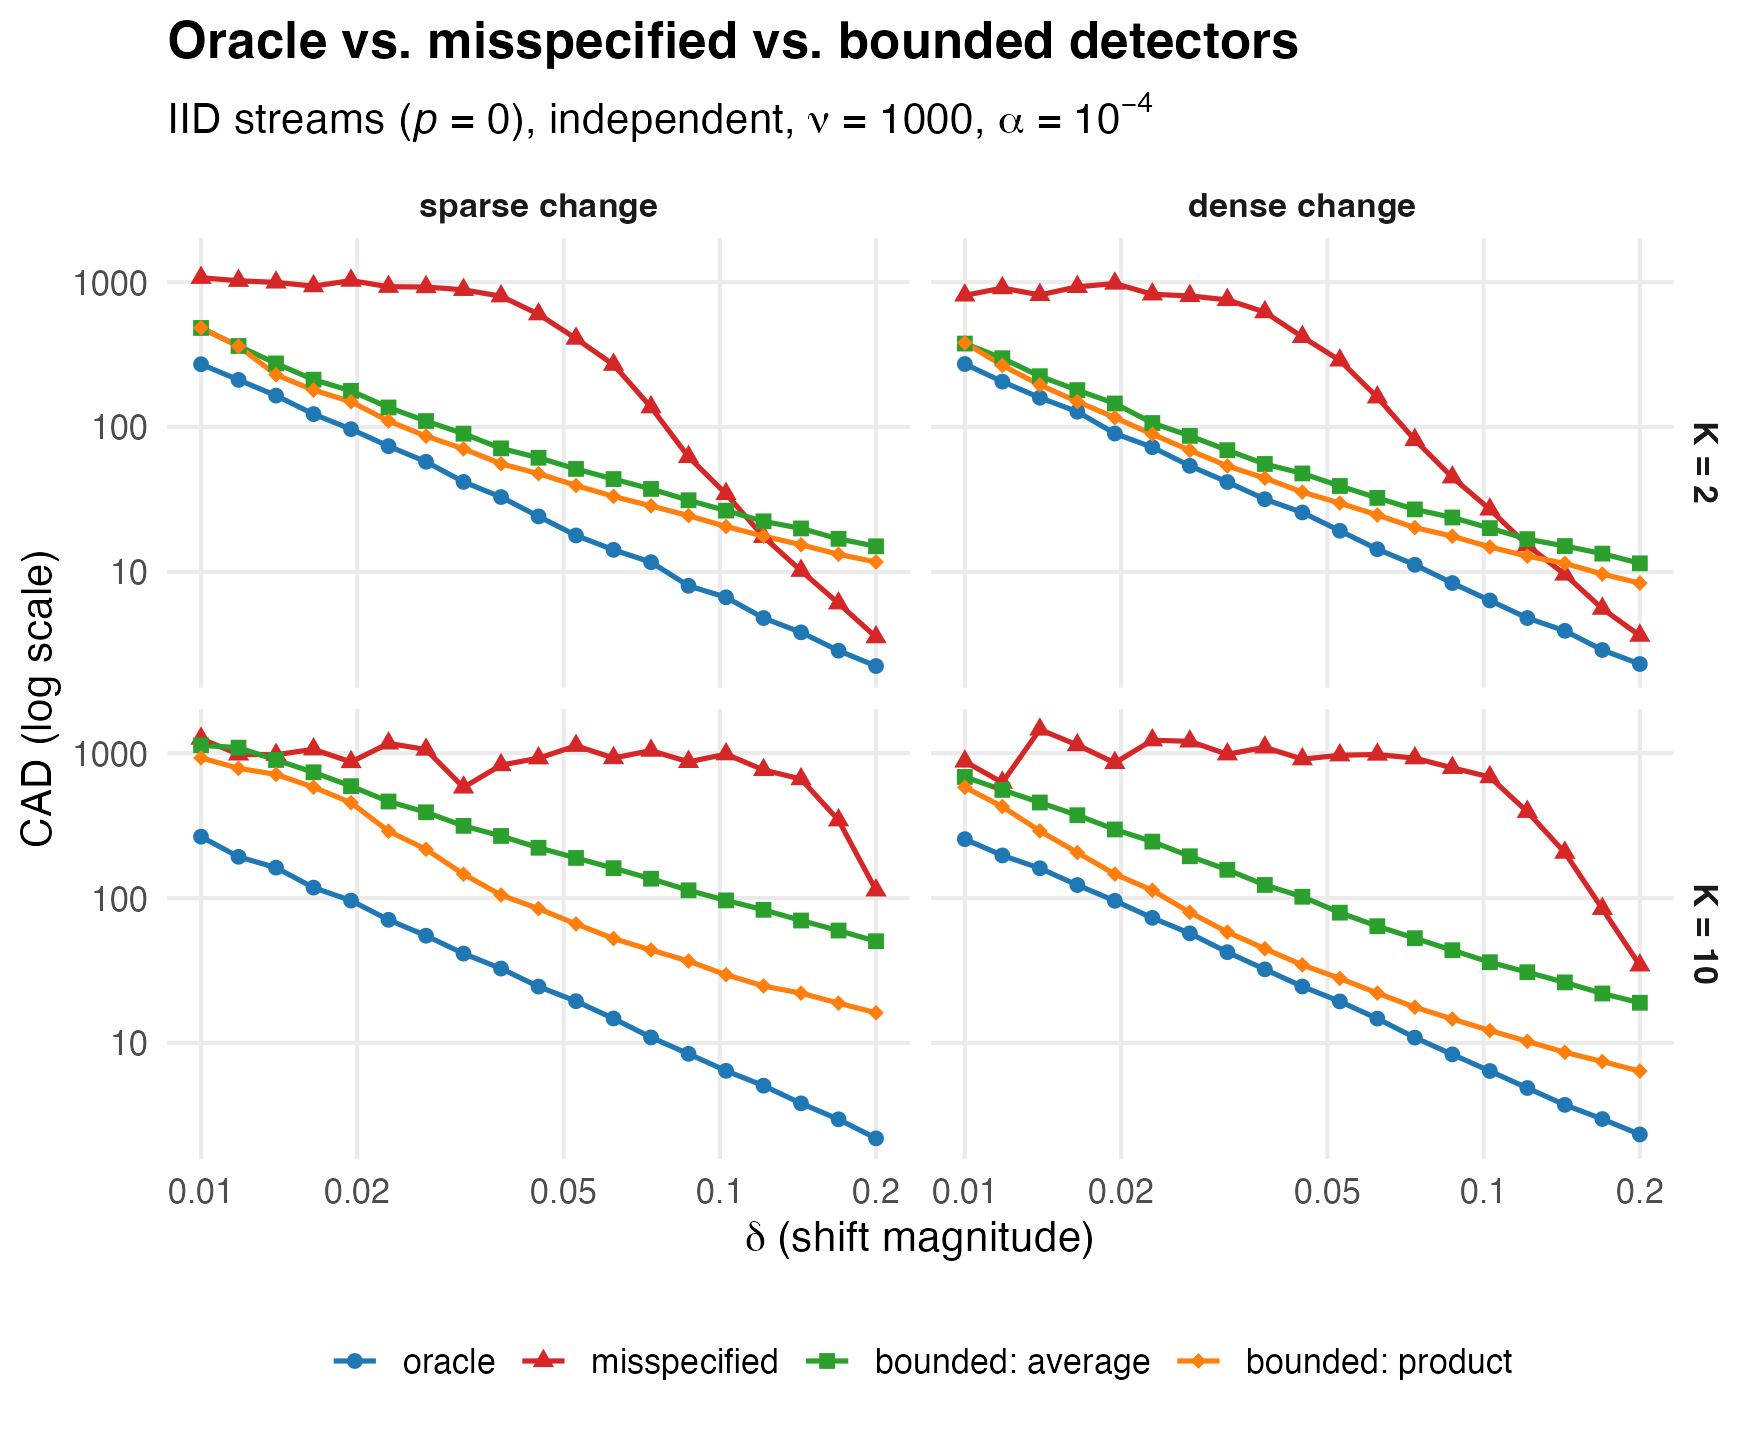
\includegraphics[width=\textwidth]{ssc-2026/figures/simulations/cad/joint_oracle_vs_bounded.png}
  \caption{Conditional average delay (CAD) of the oracle, misspecified, and bounded
    (average- and product-combined) detectors as a function of the shift magnitude $\delta$,
    faceted by number of streams $K$ and by sparse vs.\ dense change. IID streams ($p=0$),
    independent streams, $\nu = 1000$, $\alpha = 10^{-4}$.}
  \label{fig:joint-oracle-vs-bounded}
\end{figure}


% ----------------------------------------------------------------------------
% NEW subsection: betting-strategy comparison (bounded_simulations.R, Section A)
% Suggested placement: end of Section 7 (after 7.2 Localization), as 7.3;
% renumber to fit your section structure.
% ----------------------------------------------------------------------------

\subsection{Betting-strategy comparison}
\label{sec:betting-strategies}

Section~6.2 builds the bounded detector's per-stream TSM from a predictable bet sequence
$(\lambda_{tk})$, and notes a tradeoff between statistical and computational efficiency: a
detector that recomputes AGRAPA bets on the delayed TSM $M_t^{(i)}$ from each starting index $i$
adapts quickly after a change but costs $O(t^2/2)$ per stream, while a single online sequence is
cheap but ``burns in'' to the pre-change distribution and adapts slowly. Before fixing
EWMA-AGRAPA as the default for the multistream simulations of Section~7.1, we compare five betting
strategies for a single bounded stream, isolating their statistical (CAD) and computational
(wall-clock) performance as a function of the post-change mean shift $\delta$.

The data-generating process is univariate and bounded on $[0,1]$: pre-change observations are
$\mathrm{Uniform}(0,1)$ (mean $\eta = 0.5$), and post-change observations are
$\mathrm{Beta}(4(0.5+\delta), 4(0.5-\delta))$, giving a post-change mean of $0.5 + \delta$ for
$\delta \in \{0.05, 0.10, 0.15, 0.20, 0.30, 0.40\}$. The change occurs at $\nu = 50$ within a
horizon of $N = 500$ observations, and all detectors control the ARL at level
$1/\alpha = 1000$. We compare:
\begin{itemize}
  \item \textbf{Full AGRAPA} --- the AGRAPA bet of Waudby-Smith and Ramdas (2024) computed from
    the complete history since the detector started (no windowing).
  \item \textbf{Window AGRAPA ($W=30$)} --- the same AGRAPA formula restricted to the most recent
    30 observations.
  \item \textbf{EWMA ($\rho=0.10$)} --- the exponentially weighted moving-average bet of
    Section~6.2, with memory parameter $\rho = 0.1$ (an effective memory of about 10
    observations).
  \item \textbf{Per-clock ($W=30$)} --- the delayed-TSM construction described in the Remark
    following Proposition~1: rather than sharing one adaptive bet across all active clocks, each
    clock $i \le t$ recomputes its own windowed ($W=30$) AGRAPA bet from its own start time, and
    $R_t = \sum_{i=1}^t M_t^{(i)}$ is maintained directly without collapsing to a single recursion.
  \item \textbf{Oracle Kelly} --- a fixed, non-adaptive bet set to the hindsight Kelly-optimal
    value $\lambda^\star$ for the true post-change $\mathrm{Beta}$ distribution at each $\delta$.
    This strategy is infeasible in practice (it requires knowing $Q$ in advance) and serves only
    as a best-case benchmark.
\end{itemize}
Table~\ref{tab:bounded-strategy} and Figure~\ref{fig:bounded-cad-and-time} report CAD and
per-replication computation time, averaged over 500 replications per (strategy, $\delta$) cell.
Full AGRAPA is uniformly the slowest of the four feasible (non-oracle) strategies, consistent with
the burn-in effect anticipated in Section~6.2: because its bet pools pre- and post-change data
without discounting, it adapts to $Q$ more slowly than the windowed, EWMA, or per-clock
alternatives, all of which track the oracle bound closely as $\delta$ grows. Computation time is
roughly flat in $\delta$ for the four strategies that process the full length-$N$ path to build
their increments up front; the exception is the per-clock strategy, whose cost falls sharply with
$\delta$ because its recursion is evaluated online and terminates as soon as it fires, so larger
(easier to detect) shifts are simply cheaper to run to completion.

% Auto-generated by simulations/make_latex_tables.R -- do not edit by hand.
\begin{table}[t]
\centering
\caption{Conditional average delay (CAD) and per-replication computation time
  for the five betting strategies compared in the bounded-mean simulation study,
  as a function of the post-change mean shift $\delta$.
  Pre-change: $\mathrm{Uniform}(0,1)$; post-change: $\mathrm{Beta}(4(0.5+\delta), 4(0.5-\delta))$;
  $\eta = 0.5$, $\nu = 50$, $N = 500$, $\alpha = 0.001$; averages over 500 replications.}
\label{tab:bounded-strategy}
\begin{tabular}{l r rr}
\toprule
Strategy & $\delta$ & CAD & Comp.\ time (ms) \\
\midrule
\multirow{6}{*}{Full AGRAPA} & 0.05 & 156.8 & 1.67 \\
 & 0.10 & 69.7 & 1.59 \\
 & 0.15 & 45.5 & 1.54 \\
 & 0.20 & 33.3 & 1.54 \\
 & 0.30 & 21.9 & 1.51 \\
 & 0.40 & 17.9 & 1.53 \\
\midrule
\multirow{6}{*}{Window AGRAPA ($W=30$)} & 0.05 & 122.4 & 1.70 \\
 & 0.10 & 46.4 & 1.55 \\
 & 0.15 & 30.0 & 1.51 \\
 & 0.20 & 22.8 & 1.52 \\
 & 0.30 & 16.8 & 1.56 \\
 & 0.40 & 13.2 & 1.53 \\
\midrule
\multirow{6}{*}{EWMA ($\rho=0.10$)} & 0.05 & 125.3 & 2.07 \\
 & 0.10 & 45.6 & 1.97 \\
 & 0.15 & 27.0 & 1.99 \\
 & 0.20 & 19.3 & 1.99 \\
 & 0.30 & 12.9 & 2.00 \\
 & 0.40 & 10.2 & 2.01 \\
\midrule
\multirow{6}{*}{Per-clock ($W=30$)} & 0.05 & 111.8 & 3.19 \\
 & 0.10 & 42.7 & 1.78 \\
 & 0.15 & 26.5 & 1.48 \\
 & 0.20 & 19.3 & 1.31 \\
 & 0.30 & 13.3 & 1.19 \\
 & 0.40 & 10.4 & 1.16 \\
\midrule
\multirow{6}{*}{Oracle Kelly} & 0.05 & 98.8 & 1.48 \\
 & 0.10 & 37.9 & 1.47 \\
 & 0.15 & 22.6 & 1.45 \\
 & 0.20 & 16.3 & 1.49 \\
 & 0.30 & 11.1 & 1.49 \\
 & 0.40 & 8.7 & 1.49 \\
\bottomrule
\end{tabular}
\end{table}


\begin{figure}[t]
  \centering
  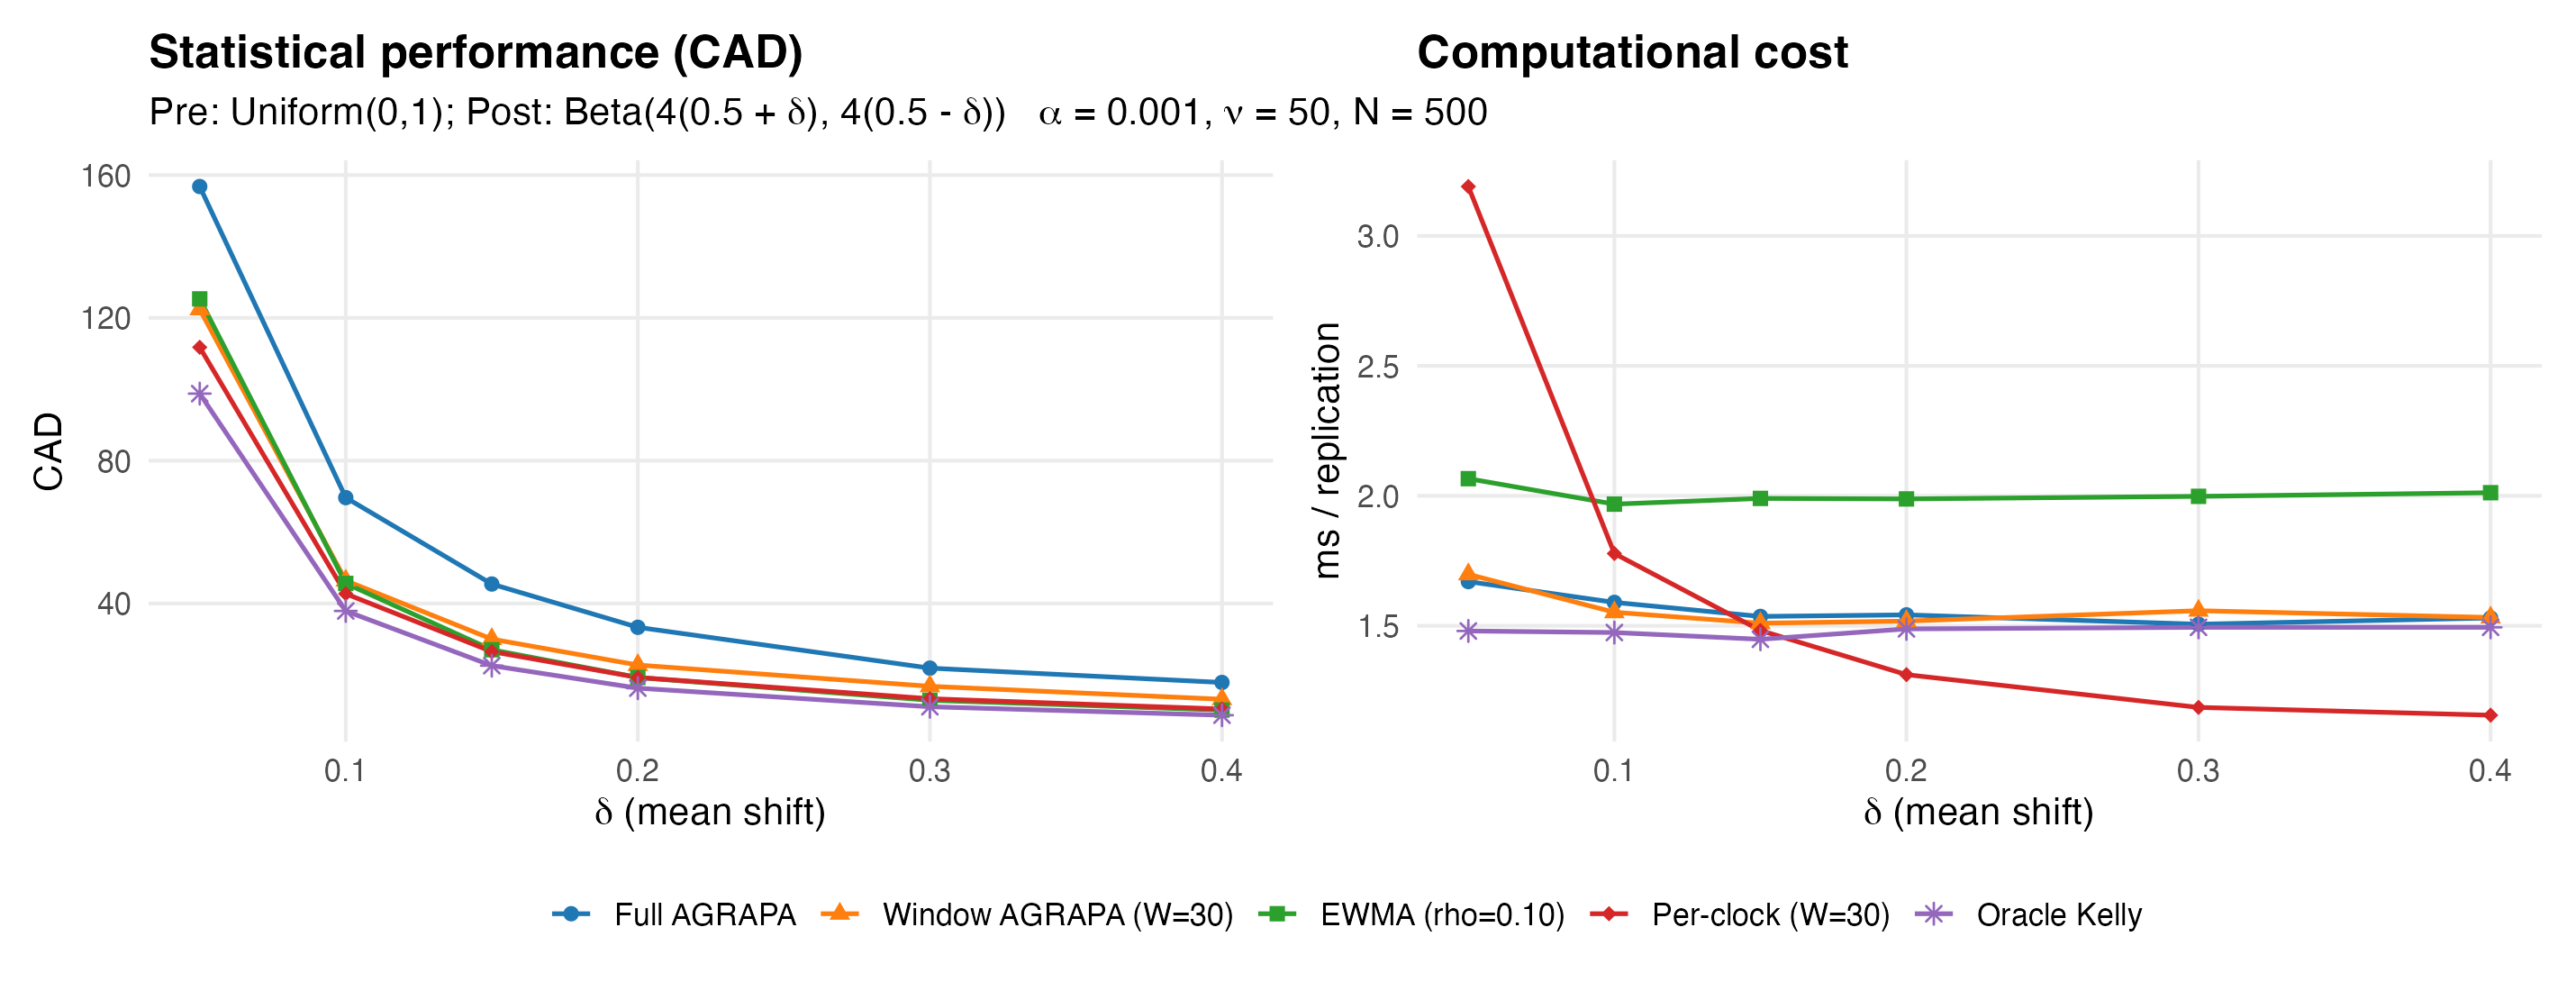
\includegraphics[width=\textwidth]{ssc-2026/figures/simulations/cad/bounded_cad_and_time.png}
  \caption{Statistical and computational performance of the five betting strategies as a function
    of the post-change mean shift $\delta$. Left: conditional average delay (CAD). Right:
    wall-clock computation time per replication. Pre-change $\mathrm{Uniform}(0,1)$; post-change
    $\mathrm{Beta}(4(0.5+\delta), 4(0.5-\delta))$; $\eta = 0.5$, $\nu = 50$, $N = 500$,
    $\alpha = 0.001$.}
  \label{fig:bounded-cad-and-time}
\end{figure}
